\documentclass[30pt,twocolumn,letterpaper]{article}
\usepackage{cvpr}
\usepackage{times}
\usepackage{booktabs}
\usepackage{epsfig}
\usepackage{graphicx}
\usepackage{amsmath}
\usepackage{amssymb}
\cvprfinalcopy
\def\cvprPaperID{****}
\def\httilde{\mbox{\tt\raisebox{-.5ex}{\symbol{126}}}}
\usepackage{graphicx}
\usepackage{indentfirst}
\setlength{\parindent}{2em}
\usepackage{cite}
\usepackage[colorlinks,linkcolor=red,anchorcolor=blue,citecolor=green,backref=page]{hyperref}
\author{Qilei Zhang}
\date{Jun 4 2018}
\title{SUNDRY TOPICS}
\begin{document}
\maketitle
\begin{abstract}
   In this section we present several topics relating to the physics of stochastic resonance that have not been featured in detail in the previous sections. In doing so, we have confined ourselves to particular examples determined only by our knowledge and personal taste; thus this selection is necessarily incomplete.
\end{abstract}
\section{Stochastic resonance in coupled systems}
we discuss the impact of noise and periodic forcing on an ensemble of coupled bistable systems. In view of a possible collective response of the system (especially close to a phase transition), one can expect that the stochastic resonance effect will be even more pronounced than in a single system\cite{Carroll1993Stochastic}.
\begin{figure}[htbp]
\small
\centering
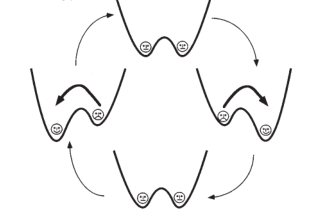
\includegraphics[width=20em]{000.png}
\caption{spatially extended systems}
\label{fig:lable}
\end{figure}
\section{Two coupled bistable systems}
The simplest way to study stochastic resonance in coupled systems is to consider two coupled overdamped bistable elements in the presence of noise and periodic forcing\cite{Collins1995Stochastic}. \\
\begin{equation}
r_n=\frac{1}{T}\int_0^T r(t)exp(-inwt)dt
\end{equation}
\begin{table}
\begin{center}
\begin{tabular}{cccccccc}
\toprule
         & 1 &  2  &   3  &  4  &  5  &  6  & 7 \\
\midrule
Alphabet & A &  B  &   C  &  D  &  E  &  F  & G\\
Roman    & I &  II &  III &  IV &  V  &  VI & VII\\
\bottomrule
\end{tabular}
\end{center}
\caption{Results ours is better.}
\end{table}
\section{Collective response in globally coupled bistable systems}
An early study dealing with stochastic resonance for systems with many degrees of freedom focused on a large number N of identical, linearly and homogeneously coupled bistable systems in the presence of periodic forcing\cite{Rallabandi2010Magnetic}.
{\small
\bibliographystyle{ieee}
\bibliography{1}
}
\end{document}
